% Drawing 156-7/04-3 -- folder 156-7, batch 04, archive page 71 (PDF page 72).
% Transcription: à la fin de la phrase, un segment subdivisé par six petits traits verticaux, extrémités comprises ; sous le premier « $a_1$ », sous le deuxième « $a_2$ », puis un point et trois tirets, et sous le dernier « $a_n$ » ; une parenthèse fermante à droite.
% Kind: subdivided segment with labelled points. Method 2 (schematic redraw from the facsimile). Status: ok.
% Notes: At the very bottom of the page, closing the sentence: a segment, rising slightly to the right, with six short vertical ticks (both ends included), placed on the line at computed points; under the first a_1, under the second a_2, then a dot and three short dashes under the following ticks, and a_n under the last; the closing parenthesis of the sentence to the right, kept because the transcription's mark names it. The subscript of the last label is read n after the text (a_1 < a_2 < ... < a_n). Nothing struck. Redrawn rather than encoded: a plain subdivided segment. Redrawn 2026-11-10 (issue 128): to check again.
% Coordinates: 1 unit = 1 mm = 1/100 of the crop width (bbox in page fractions: [0.39, 0.835, 0.82, 0.875]).
% Redrawn by Claude (claude-fable-5-2), issue #128, 2026-11-10; not checked by a human; not compiled (no TeX in the session).
% Rights: reproduces part of the work -- behind RENDER_TRANSCRIPTS, never published by itself.
\documentclass[tikz,border=3pt]{standalone}
\usepackage{amsmath,amssymb}
\usetikzlibrary{patterns,arrows.meta}
\tikzset{pencil/.style={black!45}, struck/.style={black!35}, mpt/.style={circle,draw,inner sep=1.3pt}, pt/.style={circle,fill,inner sep=0.9pt}, opt/.style={circle,draw,fill=white,inner sep=1.1pt}}
\begin{document}
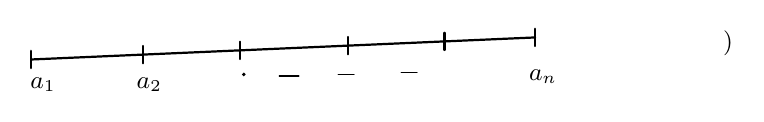
\begin{tikzpicture}[x=1mm,y=1mm,line cap=round,line join=round,font=\small]
\draw[thick] (5.5,-7.1) -- (69.5,-4.3);
\draw[thick] (5.5,-6) -- (5.5,-8.2);
\draw[thick] (19.7,-5.38) -- (19.7,-7.58);
\draw[thick] (32,-4.84) -- (32,-7.04);
\draw[thick] (45.7,-4.24) -- (45.7,-6.44);
\draw[thick] (58,-3.7) -- (58,-5.9);
\draw[thick] (69.5,-3.2) -- (69.5,-5.4);
\node[inner sep=1pt] at (7,-10.3) {\small $a_1$};
\node[inner sep=1pt] at (20.5,-10.3) {\small $a_2$};
\node[pt, inner sep=0.5pt] at (32.5,-9) {};
\draw (37,-9.2) -- (39.5,-9.2);
\draw (44.5,-9) -- (46.5,-9);
\draw (52.5,-8.8) -- (54.5,-8.8);
\node[inner sep=1pt] at (70.5,-9.3) {\small $a_n$};
\node[inner sep=1pt] at (94,-5) {\small )};
\end{tikzpicture}
\end{document}
